
\documentclass[a4paper, 12pt, onecolumn, oneside]{report}

\usepackage{geometry} 
\geometry{a4paper} 
\usepackage{graphicx} 
\usepackage{float}
\usepackage{wrapfig} 
\usepackage{lipsum} 
\usepackage  [utf8] {inputenc}
\usepackage  [portuguese] {babel}
\linespread{1.2}
%\setlength\parindent{0pt} 
\graphicspath{{./Imagens/}} 
\usepackage{graphicx}
\begin{document}
\begin{titlepage}

\newcommand{\HRule}{\rule{\linewidth}{0.4mm}}
\center 


\begin{figure}[H] 
\center{
\includegraphics[width=1.0\linewidth]{UA1}}
\end{figure}


\textsc{\ Departamento de Electrónica, Telecomunicações e Informática
 }\\[0.9cm] 

{\raggedright \textbf{Curso:} [8240] Mestrado Integrado em Eng. de Computadores e Telemática

\textbf{Disciplina:} [47137] Introdução à Eng. de Computadores e Telemática

\textbf{Ano lectivo:} 2012/2013 \\[1cm] 

}


\HRule \\[0.1cm]
{ \huge \bfseries Relatório da Aula Prática 10 \\
[0.4cm]  
Programação do Robô \\ [0.4cm] DETI PIC }\\[0.4cm] 
\HRule \\[1cm]

\begin{minipage}{0.4\textwidth} 
\begin{flushleft} \large
\emph{Autores:}\\
{[68535] Bruno \textsc{Silva}} \\
{[68799] Rui \textsc{Oliveira} } 


\emph{Turma/Grupo:}\\
T5B / Prática 3\\

\end{flushleft}
\end{minipage}
~
\begin{minipage}{0.4\textwidth}
\begin{flushright} \large
\emph{Docentes:} \\
André \textsc{Zúquete} \\
João \textsc{Barraca} \\
\emph{Data:} \\
\today 
\end{flushright}
\end{minipage}\\[2cm]



\vfill 

\end{titlepage}



\vspace*{\fill}



\textbf{Resumo:}


\begin{flushleft}

 Pretende-se através deste relatório expor sob forma escrita, o nosso desempenho e objetivos alcançados na aula de Introdução à Engenharia de Computadores e Telemática sobre a programação do robô DETI PIC, desenvolvido pelo Departamento de Eletrónica, Telecomunicações e Informática da Universidade de Aveiro.

\end{flushleft}


\vspace*{\fill}

\newpage




\newpage

\renewcommand*\contentsname{Índice}

\tableofcontents 


\newpage
 
\section{Introdução} 


Como sabemos, um robô é um dispositivo, ou conjunto de dispositivos, eletromecânicos ou biomecânicos capazes de realizar uma determinada funcionalidade de forma independente, para isso terá de ser pré-programado, ou então controlado por um ser humano. Primordialmente os robôs foram programados para desenvolver trabalhos de baixa complexidade, como por exemplo, deslocarem-se sobre superfícies planas, interagir com obstáculos, entre outros. Atualmente, os robôs realizam tarefas muito completas, e em muitos dos casos substituindo o trabalho humano. Embora, nem sempre se tira partido de todas as capacidades do robô.

Neste relatório pretendemos demonstrar o nosso desempenho na programação do robô DETI PIC, desenvolvido pelo Departamento de Eletrónica, Telecomunicações e Informática da Universidade de Aveiro. Mais à frente iremos mostrar as principais características do robô, e alguns dos equipamentos e materiais que utilizámos para conseguir concretizar esta actividade. Para a programação de robô utilizando um software, também este desenvolvido pelo DETI, chamado \emph{DETInchanting} criado a partir de linguagem JAVA e C++ e adaptado do \emph{Enchanting}, desenvolvido para robôs da LEGO\footnote{Empresa conceituada no fabrico de brinquedos, e atualmente no desenvolvimento de robôs. }. Neste caso, necessitámos de ter conhecimentos básicos de programação em JAVA, para conseguir testar as capacidades do robô, através da implementação blocos que permitem executar operações do tipo: \emph{if}... \emph{else}...; \emph{forever}... ; \emph{repeat until}... ; entre outros. 


Ambicionamos com estes testes ao robô, neste relatório, continuar a  explorar  a movimentação do robô usando tanto os sensores de luminosidade, colocados na sua parte inferior, como os sensores de distância. Iremos também utilizar os quatro led's que o nosso equipamento possui, de modo a indicar valores de variáveis usadas pelo programa. 

No problema 1, que se encontra  apresentado na próxima secção, iremos preparar o robô de modo a desenvolver um programa "base" que irá sustentar os restantes problemas. 
Para a construção desta estrutura base, necessitamos de ter alguns conhecimentos básicos sobre numeração binária.\footnote{Sistema de numeração posicional baseado nos numeros 0 e 1.}

Na tabela seguinte encontra-se listada a conversão de decimal para binário, que teremos que saber para resolver alguns dos problemas propostos.



\begin{tabular}{|c|c|}
\hline
	Numeração decimal & Numeração binária\\
\hline
	0 & 0000\\
\hline
	1 & 0001\\
\hline
	2 & 0010\\
\hline
	3 & 0011\\
\hline
	4 & 0100\\
\hline
	5 & 0101\\
\hline
	6 & 0110\\
\hline
	7 & 0111\\
\hline
	8 & 1000\\
\hline
	9 & 1001\\
\hline
	10 & 1010\\
\hline
	11 & 1011\\
\hline
	12 & 1100\\
\hline
	13 & 1101\\
\hline
	14 & 1110\\
\hline
	15 & 1111\\
\hline
\end{tabular}


Tabela 1: Conversão de decimal para binário e vice-versa.
\\


Para além da conversão, de 0 a 15, que necessitamos de conhecer, neste caso para confirmar os valor que nos irão ser apresentados através do robô, teremos que saber a forma generalizada de como calcular o valor binário de um determinado número decimal. Para isso devemos seguir os seguintes passos: 

\begin{enumerate}
\item Dado um determinado número decimal;
\item Dividir esse número por 2;
\item Observar o resto que resulta desta divisão;
\item Dividir o resultado da divisão anterior novamente por 2;
\item Repetir o último passo  sempre que seja possível a divisão;
\item Ordenar os "vários restos" da divisão por ordem decrescente do seu cálculo.

\end{enumerate}

A figura seguinte representa o processo anteriormente descrito.



\begin{figure}[H] 
\center{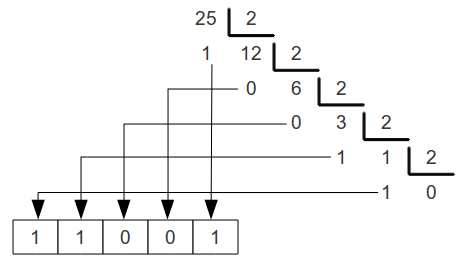
\includegraphics[width=0.8\linewidth]{binario}}
\caption{Determinar o binário de um número decimal. }
\label{fig:speciation}
\end{figure}



\newpage
\section{Descrição do problema}

Pretendemos através deste relatório dar resposta, programando e observando o comportamento do robô DETI PIC de modo a solucionar os seguintes problemas apresentados: 

\begin{itemize}
  \item \textbf{PROBLEMA 1} - Fazer um bloco que, dado um valor entre 0 e 15 mostre este valor em binário através dos quatro leds do robô. 
 
  
  

\end{itemize}


\begin{itemize}
  \item \textbf{PROBLEMA 2} -  Neste exercício pretende-se descobrir o valor de $ \Delta $ que permite equilibrar a velocidade efetiva dos dois motores do robô quando os mesmo são programados com uma velocidade base \emph{V} (ou seja, um será programado com velocidade \emph{V}, outro com \emph{V} + $ \Delta $). O valor de DELTA nunca é negativo, pelo que é preciso conhecer qual é o motor mais rápido.


Programar o robô de forma a ele seguir uma linha cuja largura é inferior à distância entre os dois sensores em torno do central (LEFT e RIGHT, no \emph{DETInchanting}). O robô deverá seguir em frente até que qualquer dos sensores de linha, pare além do central, indiquem a presença de linha. Nessa ponto deverá parar os motores (mas não o programa). O mesmo deverá acontecer no final da linha.

Seguidamente, vamos maximizar o percurso realizado pelo robô através do equilíbrio dos seus motores. Para isso vamos usar os botões de pressão para aumentar ou diminuir a diferença de velocidades entre os motores. O processo de equilíbrio dos motores deverá ser feito da seguinte forma, \textbf{sem nunca se alterar o programa}:

\begin{itemize}
  
 \item Os motores são inicialmente programado com uma velocidade igual.

 \item O robô deveá iniciar o seu percurso após sentir um obstáculo perto de um dos sensores de distância e só deverá terminar nas circunstâncias indicadas no início do exercício.

 \item Após a paragem, a diferença $ \Delta $ entre as velocidades dos motores pode ser alterada de forma a maximizar o percurso realizado. Assumindo que $ \Delta $ = $ x $ . $ \delta $,  $ x $ $ \in $ [0,7]
 e $ \delta $ $ \in $ [0,7], a alteração deverá ser feita usando os botões de pressão:
 \item Pressão curta no botão preto: $ x $ $ \longleftarrow $ $ x $ + 1
 \item Pressão longa no botão preto: $ x $ $ \longleftarrow $ $ x $ – 1
 \item Pressão curta no botão vermelho: $ \delta $ $ \longleftarrow $ $ \delta $ + 1, $ x $ $ \longleftarrow $ 0;
 \item Pressão longa no botão vermelho: $ \delta $ $ \longleftarrow $ $ \delta $ -1, $ x $ $ \longleftarrow $ 0;
\\

Este processo permite experimentar valores de $ \Delta $ desde 0 até 49, mas não todos os valores inteiros entre 0 e 49. No início da execução do programa tanto $ x $ como $ \delta $ devem ter um valor nulo.
Os valores de $ x $ e delta devem ser mostrados nos leds do robô, intervalados de 1 segundo. Como só existem 4 leds, um deles (D5) deverá ser usado para indicar qual o valor que se está a observar (desligado – $ \delta $, ligado – $ x $), e os demais para mostrar o valor (em binário).

\item O robô deverá ser novamente colocado no início da linha a percorrer e os motores deverão ser iniciados tal como no início desta sequência de passos, usando os sensores de distância. 




\end{itemize}


  \item \textbf{PROBLEMA 3} - Alterar o programa anterior para mostrar a carga da bateria, no ecrã do computador (via \emph{pterm}), no início da execução do programa (antes de fazer qualquer percurso).
Repitir o exercício anterior para várias velocidades base do robô, de modo a obter uma curva de calibração em função da velocidade base. Esta curva deverá ser apresentada no relatório, bem como o número do robô no qual ela foi observada e a carga da bateria no inicio da calibração.

\textbf{NOTA:} a carga da bateria influência a calibração. Ou seja, se a bateria tiver uma carga diferente, a curva de calibração será igualmente diferente.


\item \textbf{PROBLEMA 4} - Uma vez conhecido o $ \Delta $ apropriado para cada velocidade base, faça um programa que o explore e que siga a linha até ao seu término mas corrigindo a trajetória para maximizar o alinhamento com a linha. Este programa deverá usar os sensores de linha mais exteriores (FAR LEFT e FAR RIGHT) para detectar a presença de linhas com informação. Sempre que as detectar deverá acender um led correspondente (D5 e D2, respectivamente). 
  
 \item \textbf{PROBLEMA 5} - Alterar o programa anterior para transformar o robô num dispostivo de leitura de informação sob a forma de linhas pretas impressas (algo similiar a um código de barras). As linhas observadas pelo sensor far left fornece o sinal de leitura de informação, qual deverá ser obtida usando o sensor far right. Deste modo, sempre que existir um linha preta à esquerda da linha de deslocamento deverá ser obtido um bit, 1 ou 0, consoante à direita haja ou não uma linha preta (ver figura abaixo). 

Durante o deslocamento do robô os leds devem apresentar a seguinte informação:

\begin{itemize}  
  \item \textbf{Lido bit 0:} apaga todos os leds durante 1 segundo.
   \item \textbf{Lido bit 1:} acende todos os leds durante 1 segundo.
   
\end{itemize}


\begin{figure}[H] 
\center{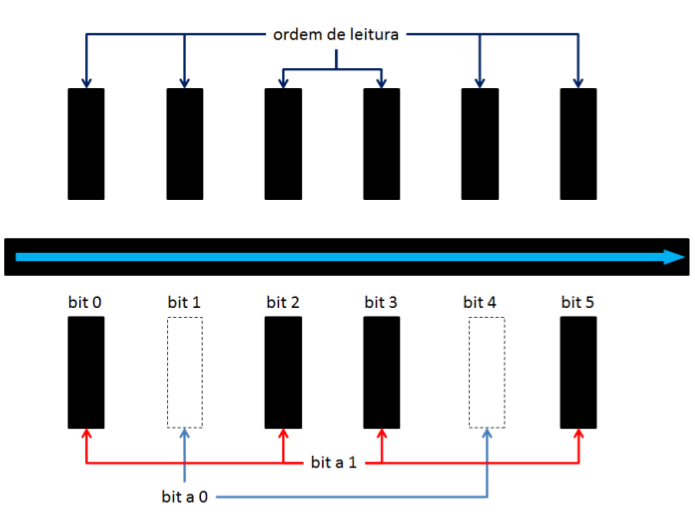
\includegraphics[width=0.7\linewidth]{ex5}}
\caption{Diagrama de um cenário possível para o Problema 5}
\label{fig:speciation}
\end{figure}


\begin{itemize}
\item \textbf{Demais situações:} acende os dois leds centrais (D3 e D4).
\\

O robô não deverá parar o seu movimento enquanto estiver a mostrar, nos leds, a informação lida.

\textbf{NOTA:} por cada ordem de leitura dada por uma linha à esquerda não deverá ser obtido mais do que um bit, mas poderão ser feitas diversas leituras do sensor para determinar esse bit. 


\end{itemize}




\end{itemize}






Para além dos cinco problemas acima descritos, pretendemos também adquirir alguns dos conhecimentos introdutórios do funcionamento e programação da robótica utilizando para isso o \emph{DETInchanting}, programa este que iremos abordar mais à frente. Dado que nos foi imposto a realização deste relatório utilizando a linguagem tipo \LaTeX, pretendemos também desenvolver as nossas competências a nível desta linguagem, alargando assim os nossos conhecimentos já adquiridos em aulas anteriores.


\newpage
\section{Aparelhagem e equipamento}



\subsection{Robô DETI PIC}

A nossa base de trabalho é o robô DETI PIC. Este robô é constituído por dois motores DC\footnote{Corrente contínua} sem realimentação, três sensores de distância frontais cobrindo um ângulo de aproximadamente 45 graus para cada lado do robô, cinco sensores de brilho na parte inferior do robô e quatro led's na parte superior. O robô dispõe ainda de dois botões, um interruptor e uma porta USB. Todo este robô foi desenvolvido de forma prática e intuitiva à introdução à programação deste tipo de máquinas. 
Para fazer o upload entre o robô e o computador utilizá-mos um cabo USB\footnote{Universal Serial Bus} 2.0.



\begin{figure}[H] 
\center{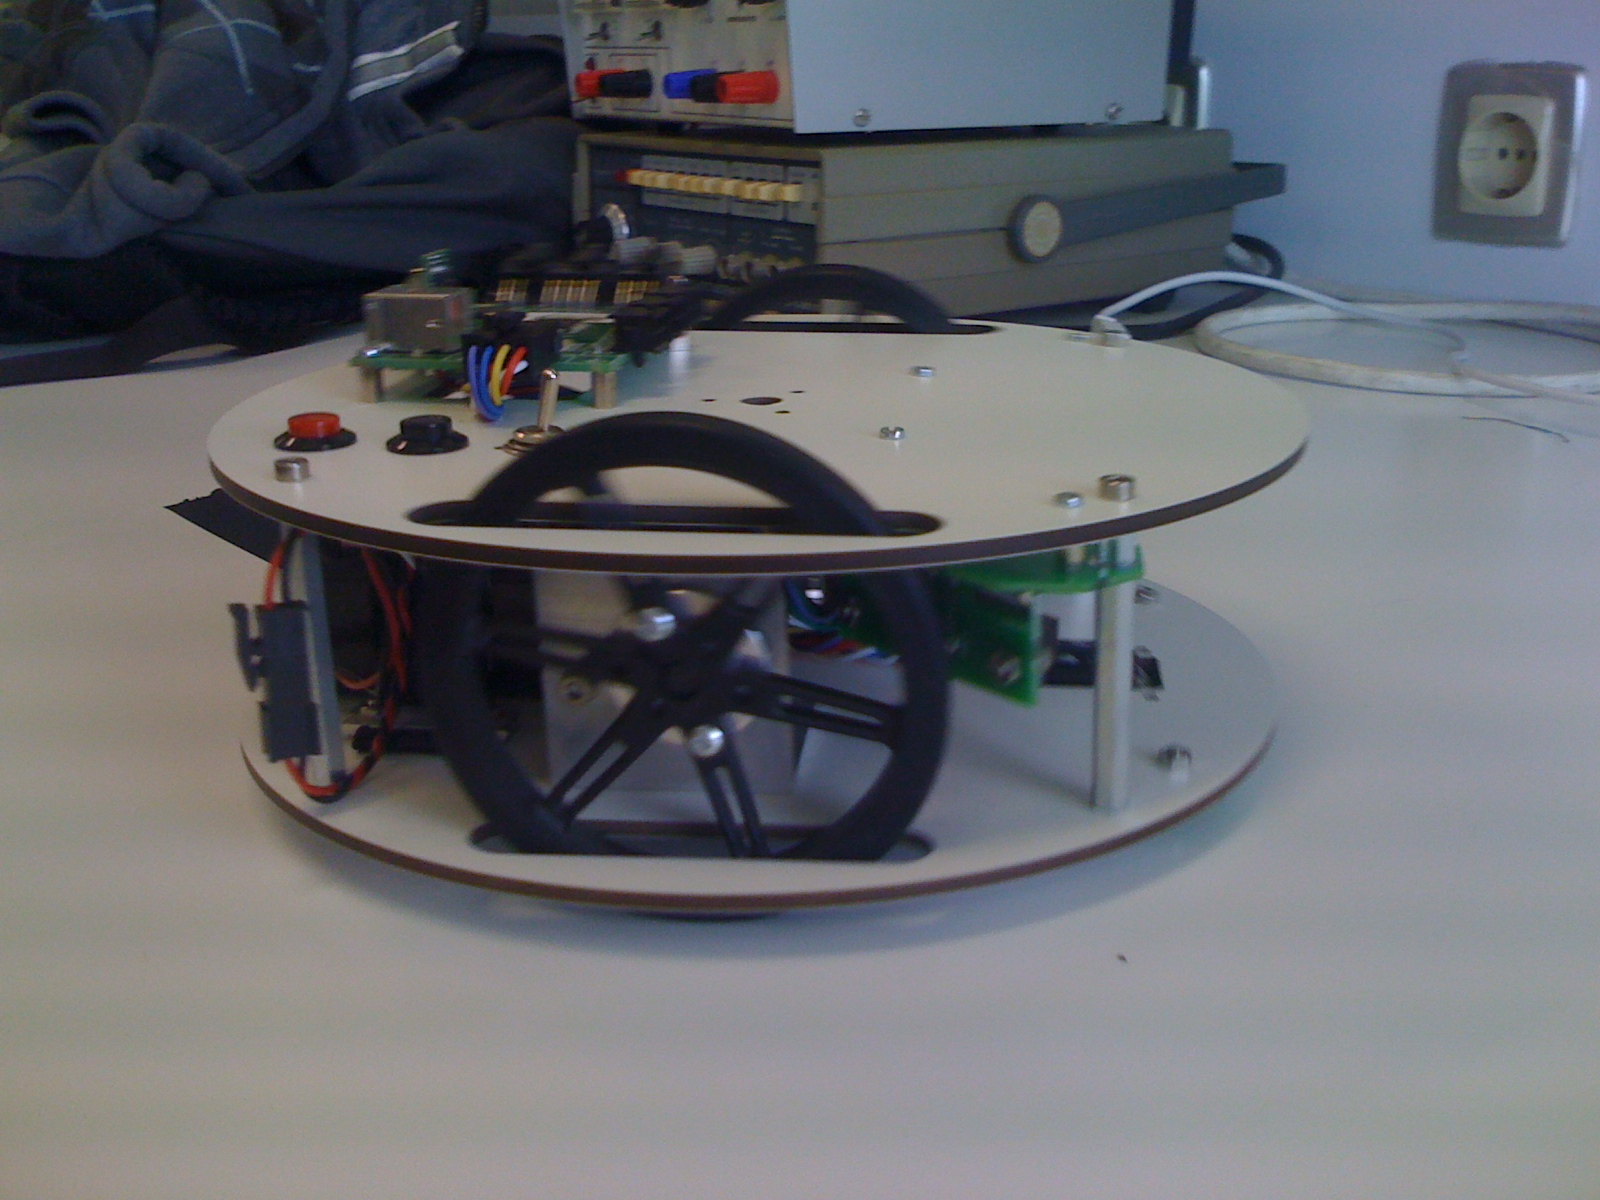
\includegraphics[width=0.5\linewidth]{robo1}}
\caption{Robô DETI PIC}
\label{fig:speciation}
\end{figure}


\subsection{Software DETInchanting}

O programa usado para a programação de instruções a dar ao robô neste trabalho foi o \emph{DETInchanting}, uma adaptação do original \emph{Enchanting} usado para programar robôs da LEGO. Este interface foi desenvolvido na Universidade de Aveiro com a intenção de facilitar a programação dos robôs utilizando um interface gráfico que se baseava em encaixes de blocos de código JAVA, na Figura 2 está representada o ambiente de trabalho deste programa. Este sofware usa um paradigma gráfico do tipo Scratch\footnote{São interfaces gráficos que permitem que programas sejam criado através da sobreposição de blocos, tendo na sua base linguagens de programação.}.



\begin{figure}[H] 
\center{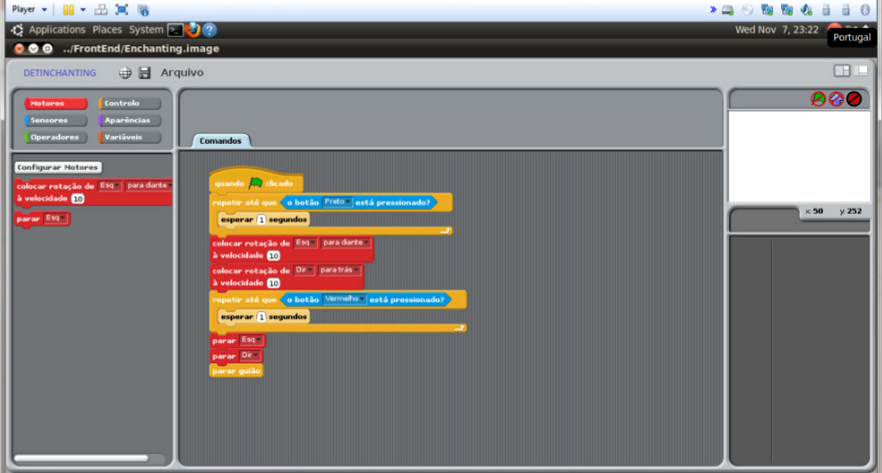
\includegraphics[width=0.9\linewidth]{ambiente}}
\caption{Ambiente do \emph{DETInchanting.}}
\label{fig:speciation}
\end{figure}




\subsection{Materiais utilizados}

O nosso ambiente de trabalho foi a bancada dos laboratórios do DETI, o que não nos dava muito espaço para manobrar o robô. Nestas condições usamos uma folha A3 com o esquema apresentado na Figura 2 da Descrição do Problema impresso. Este foi o único material que utilizámos para a resolução dos problemas apresentados, juntamente com os esquipamentos já acima referidos. 
 
 



 \newpage
 
\section{Procedimento}

\subsection{Problema 1}

Neste programa pretendemos fazer uma calibração ao robô para tornar o seu comportamento mais equilibrado e, de modo a servir como base para os restantes programas.

Começámos por criar uma função a que atribuímos o nome de “binLeds”. Esta função irá passar como argumento a variável “valor”, que foi posteriormente criada, tal como as variáveis “cont”, e “bit”. Após a criação da função, inicializámos um contador (“cont”) a zero, através do bloco “\textbf{set cont to 0}”, depois introduzimos um bloco que nos permite que todos os leds, nesta etapa do programa, estejam desligados.  Depois criámos um ciclo repetitivo “\emph{repeat until}” com a condição “\textbf{valor = 0}” ou seja a variável terá o seu início em zero. No final do ciclo, é incrementada uma unidade ao “cont”, de seguida tem-se que “\textbf{set bit to valor mod 2}”, nos irá permitir calcular o resto da divisão do valor, e "\textbf{set valor to valor / 2}", nós permitirá determinar qual será o próximo valor a que teremos que determinar novamente o resto. Desta forma conseguimos determinar a numeração binária de um determinado número, tal como demonstrámos e exemplificámos na Introdução. Quando o resto da divisão “bit” é igual à unidade então, serão ligados os led’s correspondentes ao “cont”, devidamente incrementados, no caso da primeira interação não será ligado nenhum led.

No programa principal começámos por introduzir um bloco “\emph{when clicked}” que dará inicio ao programa. Pelo facto de no início da criação do programa existirem problemas de sincronização dos leds, decidimos introduzir três blocos que nos permitem acender os mesmos durante 1 segundo, mais tarde verificámos que o problema estaria na função, que foi posteriormente corrigida.

Para finalizar introduzimos um ciclo repetitivo, no qual iremos “chamar” a função “binLeds” de modo a esta decorrer até ao “valor” 16, no final do ciclo estará presente um bloco que nos permitirá incrementar uma unidade à variável “valor” (daí a atribuição do valor 16 em vez de 15). Anteriormente ao ciclo “\emph{repeat until}” inicializámos a variável “valor” a zero através do bloco “\emph{set valor to 0}”. 



\newpage

\subsection{Problema 2}


Neste programa começámos com um ciclo \emph{forever}, onde se encontra no seu interior um \emph{if} que basicamente avalia a pressão efectuada no botão preto onde onde incrementa o $ x $ por uma unidade e de seguida altera o $\Delta$ (Delta) sendo ele o produto entre o valor actual de $x$ com o $\delta$ (delta) . A próxima condição \emph{if} avalia o mesmo procedimento mas para o botão vermelho. O código não pode ser acabado a partir deste ponto por falta de tempo, embora ainda assim tenhamos adicionado um ultimo \emph{if} que fazia o robô andar com velocidade constante no motor esquerdo e a velocidade do motor direito ia sendo alterada de modo a que fosse igualar a do motor esquerdo.



 \newpage
\section{Resultados}

\subsection{Problema 1}

Através da implementação, criação e posterior uploud do programa apresentado na Figura 5 e 6, conseguimos obdecer ao enunciado do Problema 1.

\begin{figure}[H]
\center{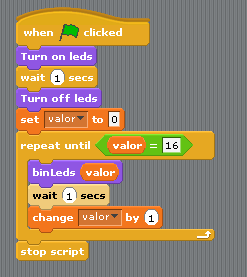
\includegraphics[width=0.4\linewidth]{1}}
\caption{Programa relativo ao problema 1.}
\label{fig:speciation}
\end{figure}


\begin{figure}[H]
\center{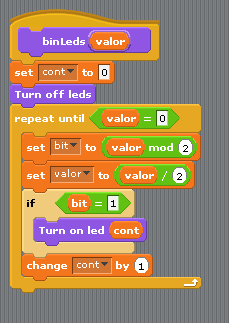
\includegraphics[width=0.3\linewidth]{f1}}
\caption{Função "binLeds" presente no programa 1.}
\label{fig:speciation}
\end{figure}



\subsection{Problema 2}

Através da implementação, criação e posterior uploud do programa apresentado na Figura 7, conseguimos obdecer, a parte do enunciado do Problema 2, embora com algumas dificuldades. 

\begin{figure}[H]
\center{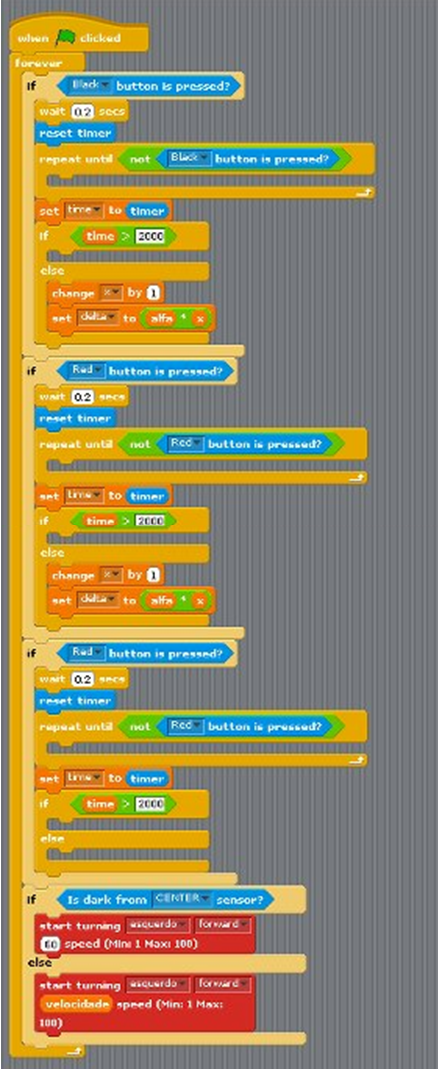
\includegraphics[width=0.4\linewidth]{2}}
\caption{Programa relativo ao problema 1.}
\label{fig:speciation}
\end{figure}



\subsection{Problemas 3, 4 e 5}

Devido à falta de tempo, não nos foi possível realizar e programar os algoritmos relativos aos problemas 3, 4 e 5, do guião a que equivale este relatório.

\newpage
\section{Análise dos Resultados}


\subsection{Problema 1}

Inicialmente, neste problema pensávamos que poderíamos criar blocos para cada número decimal, ou seja de 0 a 15. Na verdade isso era possível, mas o programa iria tornar-se demasiado extenso e com possibilidade de dificuldade na execução. O nosso docente da aula prática solicitou-nos que criássemos uma função de modo que o programa se torna-se mais legível, e mesmo extenso. Com base na informação apresentada na Introdução (como determinar o número binário de um decimal), criámos o algoritmo apresentado na secção anterior. Embora tenhamos tido algumas dificuldade na implementação dos blocos, no final conseguimos atingir o resultados que pretendemos, sem grandes erros, estes foram posteriormente corrigidos.
Na figura apresentada de seguida, está esquematizado o decorrer do programa em função do tempo. A cor amarelo (representado a luz acesa do led) e a branca (representado a luz apagada do led), correspondem respectivamente ao valor 1 e 0 da numeração binária. Conforme a Tabela 1 apresentada na Introdução observámos os mesmo resultados no robô, tal como esperávamos.



\begin{figure}[H]
\center{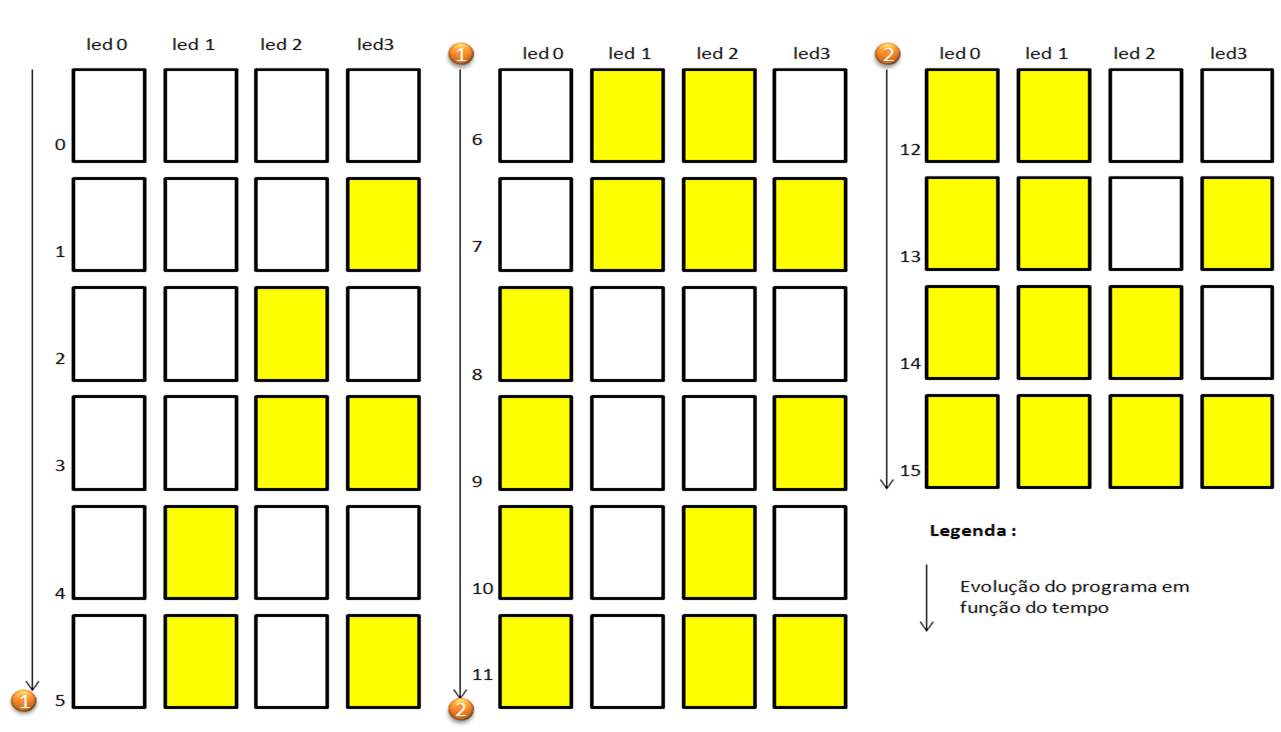
\includegraphics[width=1.0\linewidth]{leds}}
\caption{Esquema relativo ao Problema 1.}
\label{fig:speciation}
\end{figure}



\subsection{Problema 2}


Este problema foi o que nos causou maior dificuldade um pouco pela complexidade mas também pelo tempo que tínhamos para a resolução. Com isto e devido muito à “pressa” de acabar o programa fizemos muitos erros que facilmente eram corrigidos ou mesmo evitados com mais tempo. Erros esses como o não ter atribuído a variável velocidade à velocidade inicial mais o $\Delta$ (delta) e depois ter usado essa variável no motor direito. Outro erro foi o ter colocado o mesmo motor a andar sendo um deles o direito e outro o esquerdo, e por último os motores deviam estar os dois dentro do ultimo \emph{if} e não separados estando um no \emph{else}.
Concluindo não consideramos este programa como um resultado positivo mas achamos que embora tenha algum nível de complexidade poderíamos ter resolvido com um pouco mais de tempo.



 \newpage

\section{Conclusões}

Chegado ao final deste relatório, é nossa intenção efetuar uma retrospetiva da evolução do mesmo, tendo em conta os problemas que nos deparámos, objetivos, e principais metodologias utilizadas.

Apesar de não termos consigo testar e programar todos os problemas apresentamos na integra, devido ao fator tempo, pensamos que os problemas "base" foram bem conseguido, embora o ultimo com algumas dificuldades, que já frisámos em secções anteriores. 


Achámos sem qualquer dúvida, que a programação do robô DETI PIC deu-nos bastante gozo e interesse a programar, dando-nos assim uma grande introdução aos conhecimentos sobre a programação em robótica. Na nossa opinião, esta disciplina foi uma mais valia não só devido a estes conhecimentos aprendidos, anteriormente citados, mas principalmente devido à introdução na aprendizagem da linguagem \LaTeX.







\begin{thebibliography}{99} 

\bibitem[1]{Figueredo:2009dg}
A.V.C.M. Zúquete , Site da Unidade Curicular - Introdução à Engenharia de Computadores e Telemática (18 Dezembro 2012).
\newblock Diapositivos: robô DETI PIC [Online]
\newblock {\em Available: } http://www.ieeta.pt/~avz/Aulas/IECT/12-13/docs/6-robo.pdf 

\bibitem[2]{Figueredo:2009dg}
J. Barraca, D. Gomes, A. Zúquete , Site da Unidade Curicular - Introdução à  Engenharia de Computadores e Telemática (18 Dezembro 2012).
\newblock Guião da aula prática 10 [Online]
\newblock {\em Available: } http://www.ieeta.pt/~avz/Aulas/IECT/12-13/docs/guiao-10.pdf 

 
\end{thebibliography}


\end{document}
